\documentclass[10pt,conference,compsocconf]{IEEEtran}

\usepackage{hyperref}
\usepackage{graphicx}	% For figure environment

% Packages added by Joachim

%drow graph
\usepackage{fancybox}
\usepackage{tikz}
\usepackage{capt-of}
\usepackage{verbatim}

% cancel math expression
\usepackage{cancel}

% math
\usepackage{amsmath}


\begin{document}
\title{PCML CS-433: Higgs Challenge Project}

\author{
  Joachim Muth, SCIPER 214757, joachim.muth@epfl.ch\\
  Junze Bao, SCIPER 266983, junze.bao@epfl.ch\\
  Chanhee Hwang, SCIPER 260872, chanhee.hwang@epfl.ch\\ \\
  \textit{School of Computer and Communication Sciences, EPF Lausanne, Switzerland}
}

\maketitle

%========================
\begin{abstract}
...
\end{abstract}

%========================
\section{Introduction}
The ATLAS experiment consists of collisions between protons. Particles created by these collisions are detected by sensors, producing a sparse vector of about a hundred thousand dimensions. Analyzing these data, ATLAS team try to estimate if the detected particles comes from a Higgs boson decay.

The \emph{Higgs boson machine learning challenge} consists of a large dataset of particles decay detections labeled as Higgs or background. The dataset is composed of thirty features and is already cleaned from a lot of well-known background effect well-known by the ATLAS team. Also, in order to balance the great number of background events compared to Higgs events, the size of both dataset is balanced.~\cite{higgsChallenge}

%========================
\section{Models and Methods}

\subsection{Standardization}
{\color{red}DO WE REALLY NEED IT ????}\\
In order to work on comparable data, and not to overweight some of them, a standardization must be applied on them.

\subsection{Split of the data}
In order to chose which features to keep in the machine learning modelling we did, and to deal with the great number of \emph{NaN} in the data set, we analyzed their distrubution. 

It show that it's possible to cathegorize the events into four different sets based on the number of jets (\emph{int} $\in [0, 3]$). There is a physics reason behind it, since some measures make no sens for some jet numbers. \cite{higgsChallenge}.

Once this split proceeded, subsets share all the same defined features, except the estimated mass $m_H$ of the Higgs boson candidate. Once again, these subsets are split into two subsets to obtain, finally, eight different subsets to model (see figure \ref{split})

\begin{figure}[tbp] %-------TIKZ PICTURE---------
  \centering
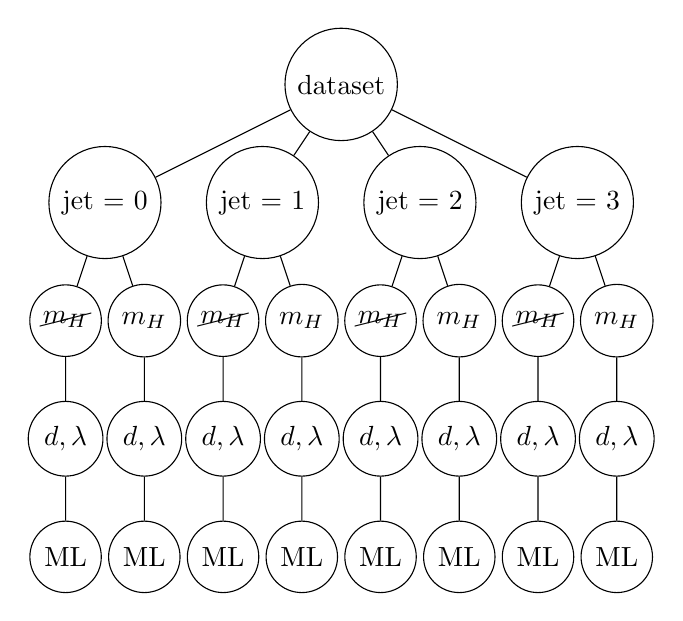
\begin{tikzpicture}[level/.style={sibling distance=20mm/#1}]
\node [circle,draw] (z){dataset}
  child {node [circle,draw] (j) {jet = 0}
  child {node [circle,draw] (l) {$\cancel{m_H}$}
    child {node [circle,draw] (c){$d, \lambda$}
      child {node [circle,draw] (p) {ML}
      }
    }
  }
  child {node [circle,draw] (l) {$m_H$}
    child {node [circle,draw] (c){$d, \lambda$}
      child {node [circle,draw] (p) {ML}
      }
    }
  }
}
  child {node [circle,draw] (j) {jet = 1}
  child {node [circle,draw] (l) {$\cancel{m_H}$}
    child {node [circle,draw] (c){$d, \lambda$}
      child {node [circle,draw] (p) {ML}
      }
    }
  }
  child {node [circle,draw] (l) {$m_H$}
    child {node [circle,draw] (c){$d, \lambda$}
      child {node [circle,draw] (p) {ML}
      }
    }
  }
}
  child {node [circle,draw] (j) {jet = 2}
  child {node [circle,draw] (l) {$\cancel{m_H}$}
    child {node [circle,draw] (c){$d, \lambda$}
      child {node [circle,draw] (p) {ML}
      }
    }
  }
  child {node [circle,draw] (l) {$m_H$}
    child {node [circle,draw] (c){$d, \lambda$}
      child {node [circle,draw] (p) {ML}
      }
    }
  }
}
  child {node [circle,draw] (j) {jet = 3}
  child {node [circle,draw] (l) {$\cancel{m_H}$}
    child {node [circle,draw] (c){$d, \lambda$}
      child {node [circle,draw] (p) {ML}
      }
    }
  }
  child {node [circle,draw] (l) {$m_H$}
    child {node [circle,draw] (c){$d, \lambda$}
      child {node [circle,draw] (p) {ML}
      }
    }
  }
};
\end{tikzpicture}
  \caption{Overall view of modelling pipeline. Split of the dataset into eight different cathegories, search of 
  the parameters and calculation of weight by Ridge Regression.}
  \vspace{-3mm}
  \label{split}
\end{figure}




\subsection{Features selection}
{\color{red} WE MUST TEST IT AND CHOSE IF WE KEEP} \\
As our eight datasets are well splitted, we can just discard the features only containing \emph{NaN} values. The remaining features are well completed. This does not mean that they are all interesting. The histogram of their frequencies show candidates of possibly useless features which have almost no variance (see figure \ref{hist})

\begin{figure}[tbp] %-------TIKZ PICTURE---------
  \centering
  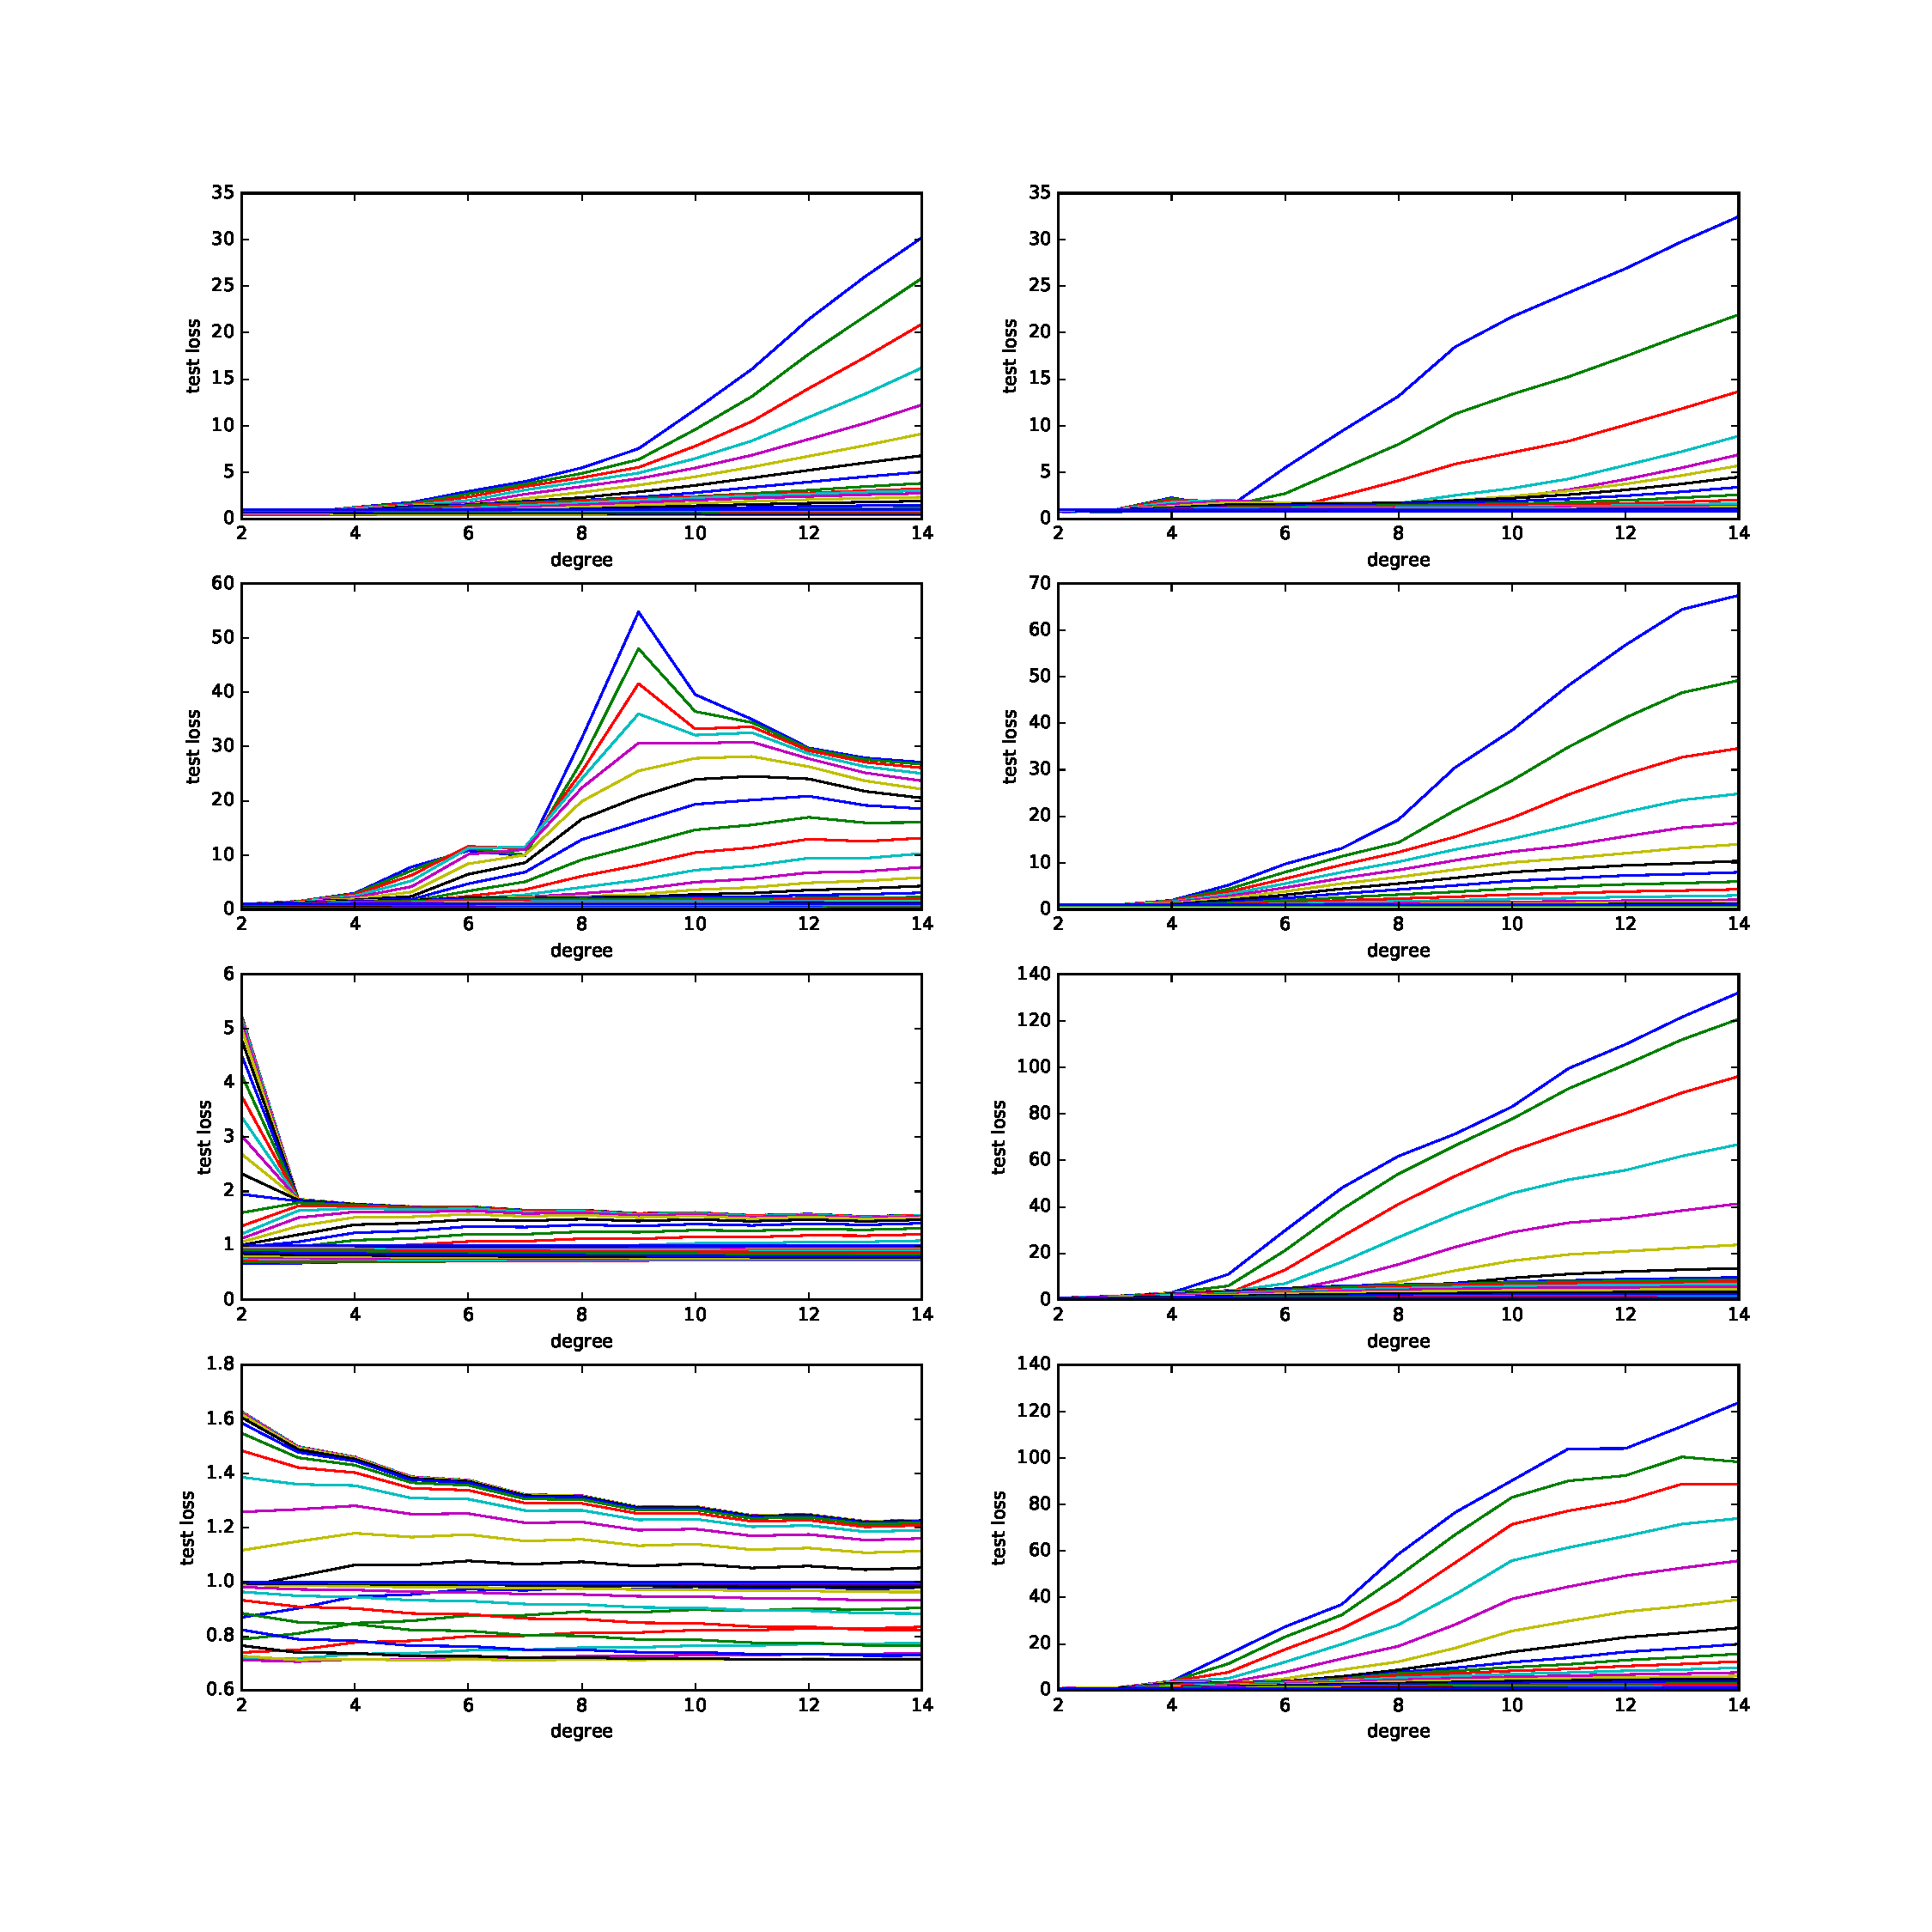
\includegraphics[width=\columnwidth]{img/cross_validation_lot.pdf}
  \caption{Grid search for parameter selection $d$ and $\lambda$ on the eight data subsets. }
  \vspace{-3mm}
  \label{param}
\end{figure}


\subsection{Polynomial building}
We construct a polynom matrix of degree $d$ with our features matrix. The degree is chosen by 4-fold cross validation and is different for each of our eight datasets.


\subsection{Selection of Ridge Regression parameters}
We apply a 2-steps grid-search method on each of the eight data subset for two parameters: \textbf{polynomial degree} $d \in [0, 15]$ and \textbf{regularization parameter} $\lambda \in [1^{-10}, 1]$.  Each pair of parameter is test through a 4-fold cross-validation and scored by RMS error. Figure \ref{param} shows the result. Once the best parameters are chosen for each subsets, we zoomed on them and apply again a grid-search on the zoomed interval, to gain precision. Table \ref{tab:param} sums up the chosen parameters.

\begin{table}[htbp]
  \centering
  \begin{tabular}[c]{| l| | c | c |}
    \hline
    Subset 	& lambda $\lambda$ & degree $d$ \\
    \hline \hline
    jet0 no mass 			& 1.5998e-05	& 2		\\
    jet0 mass 				& 3.2374e-05	& 2		\\
    jet1 no mass				& 0.1526		& 13 		\\
    jet1 mass				& 3.2374e-05 	& 2 		\\
    jet2 no mass				& 0.0184		& 2		\\
    jet2 mass				& 7.9060e-06	& 3		\\
    jet3 no mass				& 0.6250		& 3		\\
    jet3 mass				& 0.0091		& 3		\\
    \hline
  \end{tabular}
  \caption{Selected parameters of Ridge Regression}
  \label{tab:param}
\end{table}




%========================
\section{Results}
This model gives us an accuracy of $83.75 \%$ when tested by 4-fold cross-validation. However, the accuracy against test set provided on Kakkgle.com only scored $77.748\%$


%========================
\section{Discussion}


%========================
\section{Summary}

...


\bibliographystyle{IEEEtran}
\bibliography{literature}

\end{document}
